%%%%%%%%%%%%%%%%%%%%%%%%%%%%%%%%%%%%%%
%         PACKAGES INCLUSION         %                                                                                      % PACKAGES
%%%%%%%%%%%%%%%%%%%%%%%%%%%%%%%%%%%%%%

\documentclass[a4paper,10pt]{article}                                                                                       % Document specs
\usepackage[legalpaper, margin=2cm]{geometry}                                                                               % Document margin
\usepackage[utf8]{inputenc}                                                                                                 % Encoding specs
\usepackage{tocloft}                                                                                                        % Package import for table of contents with dots
\usepackage{abstract}                                                                                                       % Package import for abstract
\usepackage{hyperref}                                                                                                       % Package import for external references
\usepackage{graphicx}                                                                                                       % Package import to manage images labels and captions
\usepackage{cite}                                                                                                           % Package import for bibliographies (citations)
\usepackage[usenames,dvipsnames,svgnames,table]{xcolor}                                                                     % Package import for colors
\usepackage{amsmath}                                                                                                        % Package import for formulas (math)
\usepackage{amssymb}                                                                                                        % Package import for formulas (symbols)
\usepackage{chngcntr}                                                                                                       % Package import for formulas (enumeration)

%%%%%%%%%%%%%%%%%%%%%%%%%%%%%%%%%%%%%%
%           PREAMBLE START           %                                                                                      % PREAMBLE
%%%%%%%%%%%%%%%%%%%%%%%%%%%%%%%%%%%%%%

\hypersetup{
  colorlinks=true,
  linkcolor=darkgray,
  filecolor=magenta,
  urlcolor=blue,
  citecolor=gray,
  pdftitle={DataAnalysis},
  pdfpagemode=FullScreen}                                                                                                   % External references definition: dark-grey links and blue URLs (\href call)
\setlength{\parindent}{1cm}                                                                                                 % Remove indentation at paragraph's start
\renewcommand{\abstractname}{Sommario}                                                                                      % Abstract title
\renewcommand{\contentsname}{Indice}                                                                                        % Change table of contents (Toc) title
\renewcommand{\cftsecleader}{\cftdotfill{\cftdotsep}}                                                                       % Configure table of contents (Toc) to display dots
\renewcommand{\cftsecfont}{\normalsize}                                                                                     % ToC-sec font
\renewcommand{\cftsubsecfont}{\normalsize}                                                                                  % ToC-subsec font
\renewcommand{\cftsubsubsecfont}{\normalsize}                                                                               % ToC-subsubsec font
\setlength{\cftsecindent}{0mm}                                                                                              % ToC-sec indentation
\setlength{\cftsubsecindent}{2mm}                                                                                           % ToC-subsec indentation
\setlength{\cftsubsubsecindent}{4mm}                                                                                        % ToC-subsubsec indentation
\setlength{\cftsecnumwidth}{5mm}                                                                                            % ToC-sec distance from number
\setlength{\cftsubsecnumwidth}{8mm}                                                                                         % ToC-subsec distance from number
\setlength{\cftsubsubsecnumwidth}{11mm}                                                                                     % ToC-subsubsec distance from number
\renewcommand{\theequation}{{Eq.} \thesubsubsection.\arabic{equation}}                                                      % Change equations enumeration
\counterwithin*{equation}{section}                                                                                          % Restart equations enumeration at new section
\counterwithin*{equation}{subsection}                                                                                       % Restart equations enumeration at new subsection
\counterwithin*{equation}{subsubsection}                                                                                    % Restart equations enumeration at new subsubsection
\renewcommand{\tablename}{Tab.}                                                                                             % Change tables enumeration
\renewcommand{\figurename}{Fig.}                                                                                            % Change figures enumeration
\bibliographystyle{plain}                                                                                                   % Bibliography style (plain standard style)
\renewcommand\refname{Riferimenti bibliografici}                                                                            % Bibliography title

\title{Analisi dati e calcoli ingegneristici scambiatore di calore\\                                                        % Title definition (printed with \maketitle command)
\large Laboratorio - Gruppo n.5 del 26/11/2021, fisica tecnica [140078] AA 2021/2022}                                       % Subtitle definition (printed with \maketitle command)
\author{Cristian Merli, matr. 211384}                                                                                       % Authors definition (printed with \maketitle command)
\date{07/02/2022}                                                                                                           % Date definition (printed with \maketitle command)

%%%%%%%%%%%%%%%%%%%%%%%%%%%%%%%%%%%%%%
% END OF PREAMBLE and DOCUMENT START %                                                                                      % DOC-START
%%%%%%%%%%%%%%%%%%%%%%%%%%%%%%%%%%%%%%

\begin{document}                                                                                                            % Document-start

\maketitle                                                                                                                  % Plot previously defined title

\vspace{4cm}                                                                                                                % Vertical-space command
  \addcontentsline{toc}{section}{Sommario}                                                                                  % Add abstract inside table of contents
  \begin{abstract}                                                                                                          % Abstract creation and following abstract text
    \noindent \textit{Relazione sintetica con lo scopo di descrivere le scelte adottate, e discutere i risultati  ottenuti
    dall'analisi dati e dalle modellazioni ingegneristiche effettuate. Il sistema oggetto di modellazione, è costituito da
    uno scambiatore di calore a fascio tubiero, all'interno del quale scorre acqua in entrambi i circuiti di scambio. Sono
    state effettuate diverse prove, in particolare: due in configurazione equi-corrente e due in configurazione
    contro-corrente, con diversi valori di portata volumetrica di fluido freddo.\\
    Nei capitoli successivi, verranno elencate le richieste di progetto avanzate dal docente e verranno ripercorse le varie
    tappe, che hanno condotto alla realizzazione e comparazione di diversi modelli ingegneristici più o meno raffinati,
    mediante l'analisi assistita da calcolatore dei dati raccolti durante l'esperienza di laboratorio (effettuata in data
    26/11/2021 con il gruppo numero 5, presso i laboratori del dipartimanto di fisica dell'università di Trento).}
  \end{abstract}                                                                                                            % Abstract end
\vspace{2.5cm}                                                                                                              % Vertical-space command

\vspace{2.5cm}                                                                                                              % Vertical-space command
  \tableofcontents                                                                                                          % Plot table of contents
\pagebreak                                                                                                                  % Go to new page

\section{Richieste}                                                                                                         % Section creation: "Richieste"
\label{sec:project_request}                                                                                                 % "project_request" reference-label definition and following section text
  Le richieste di progetto consistono principalmente nella realizzazione di un sistema di analisi dati "computerizzato",
  per poter cogliere da esso, le informazioni necessarie ad effettuare i diversi calcoli inerenti il fenomeno di scambio
  termico. Il tutto, con l'obiettivo di caratterizzare tale fenomeno sul manufatto oggetto di analisi sperimentale. In
  aggiunta, è stato richiesto di cogliere le analogie e tutto ciò in cui i risultati teorici attesi, differiscono da
  quelli sperimentali ottenuti, con particolare attenzione in riferimento alla non adiabaticità del sistema e alle varie
  approssimazioni effettuate in fase di modellazione, per lo studio del trasferimento di calore all'interno e all'esterno
  della macchina termica.

\section{Introduzione}                                                                                                      % Section creation: "Introduzione"
\label{sec:introduction}                                                                                                    % "introduction" reference-label definition and following section text
  Per rispondere alle richieste di progetto, come riportato anche nel sommario di questo documento, è stata
  realizzata una parte di calcolo assistito con alcuni commenti per motivare e descrivere i vari passaggi effettuati.
  Questo elaborato ha quindi come unico scopo, quello di illustrare i passaggi cruciali, le scelte salienti adottate e
  discutere i risultati ottenuti nella parte tecnica. Per maggior trasparenza, è stato reso accessibile online l'intero
  codice sorgente realizzato, senza la necessità di effettuare alcuna installazione e/o configurazione dell'ambiente di
  sviluppo per poterlo consultare. Il seguente link, consente un accesso diretto alla repository di GitHub caricata
  personalmente, per poter approfondire tutto ciò che è stato realizzato:
  \textit{\href{https://github.com/CristianMerli/DataAnalysis.git}{https://github.com/CristianMerli/DataAnalysis.git}}.

\section{Linguaggio di programmazione}                                                                                      % Section creation: "Linguaggio di programmazione"
\label{sec:progr_lang}                                                                                                      % "progr_lang" reference-label definition and following section text
  Il passo preliminare per poter portare a compimento le richieste avanzate da parte del docente
  \textit{\textbf{[}Capitolo \ref{sec:project_request}, pagina~\pageref{sec:project_request}\textbf{]}}, è stato quello di
  individuare un software di "data science", per la realizzazione della parte di analisi dati e calcolo ingegneristico. La
  scelta più ovvia in ambito accademico, sarebbe stata quella di utilizzare il software MatLab, ma si è optato per un
  programma di tipo open-source, riutilizzabile anche in futuro essendo libero da licenze. É stato quindi scelto un
  linguaggio denominato python, dotato di numerosi pacchetti dedicati al "data science", tra cui pandas e numpy.
  L'ambiente di sviluppo utilizzato (IDE) è Visual Studio Code, installato su una macchina linux con un ambiente virtuale
  python dedicato allo sviluppo di tale progetto (conda environment). Un esempio di configurazione simile per analisi
  dati, può essere trovato al seguente link:
  \textit{\href{https://code.visualstudio.com/docs/datascience/data-science-tutorial}{vedi esempio}}. Infine, è stato
  utilizzato il sistema di gestione del codice "git", unitamente al servizio di hosting fornito da GitHub, con l'intento
  di pubblicare online e rendere facilmente accessibili tutti i contenuti realizzati. Il codice che compone la parte
  tecnica di questo progetto, è composto da uno script python principale di tipo JupyterNotebook e da un pacchetto
  (libreria) appositamente sviluppato, denominato "libs". Esso contiene diversi script in linguaggio nativo python, con
  compiti specifici tra cui: caricamento dati misure, esecuzione analisi dati, formule di calcolo ingegneristico,
  stampaggio a video di grafici, approssimazione polinomiale delle proprietà delle variabili termofisiche e molto
  altro.\vspace{2mm}\\
  "One of the really big growth areas for Python is in the sciences, where data analysis is a huge component."
  \textit{(by Bernard, Joey)}
  \cite{Bernard2016}

\section{Analisi dati}                                                                                                      % Section creation: "Analisi dati"
\label{sec:data_analysis}                                                                                                   % "data_analysis" reference-label definition and following section text
  L'analisi dei dati, è stata 

\section{Calcoli ingegneristici}                                                                                            % Section creation: "Calcoli ingegneristici"
\label{sec:engineering_calcs}                                                                                               % "engineering_calcs" reference-label definition and following section text
  XSAHxsjhsavxsgavsxgh

\section{Conclusioni}                                                                                                       % Section creation: "Conclusioni"
\label{sec:conclusions}                                                                                                     % "conclusions" reference-label definition and following section text
  XSAHxsjhsavxsgavsxgh

\section{Formule}                                                                                                           % Section creation: "Formule"
\label{sec:formulas}                                                                                                        % "formulas" reference-label definition and following section text
\subsection{Formule analisi dati}                                                                                           % Subsection creation: "Formule analisi dati"
\label{subsec:da_formulas}                                                                                                  % "da_formulas" reference-label definition and following subsection text
\subsubsection{Scelta miglior intervallo dati con condizioni stazionarie}                                                   % Subsubsection creation: "Scelta miglior intervallo dati con condizioni stazionarie"
\label{subsubsec:daf_interv}                                                                                                % "daf_interv" reference-label definition and following subsubsection text
\begin{equation}                                                                                                            % Equation-start
  I_{condiz.staz.} = I(s_j) : \{I(s_j) = \min_{\forall I_M \in M} s_j\}                                                     % Formula
  \qquad\text{con}\qquad                                                                                                    % Conjunction txt
  I(s_j) = \frac{1}{N}\sum_{j=1}^{m}{s_j}                                                                                   % Formula
  \qquad\text{e}\qquad                                                                                                      % Conjunction txt
  s_j = \sqrt[2]{\frac{1}{n-1}\sum_{i=1}^{n}(x_i-\overline{x})^2}                                                           % Formula
  \label{eqn:stat}                                                                                                          % Reference-label to equation
\end{equation}                                                                                                              % Equation-end
\subsection{Formule calcoli ingegneristici}                                                                                 % Subsection creation: "Formule calcoli ingegneristici"
\label{subsec:ec_formulas}                                                                                                  % "ec_formulas" reference-label definition and following subsection text
\subsubsection{Trasferimento di calore}                                                                                     % Subsubsection creation: "Trasferimento di calore"
\label{subsubsec:ecf_heat_tr}                                                                                               % "ecf_heat_tr" reference-label definition and following subsubsection text
\begin{equation}                                                                                                            % Equation-start
  Q_c = \dot{m}_c\mathcal{C}_{p,c}(T)\Delta{T_c}                                                                            % Formula
  \qquad\text{e}\qquad                                                                                                      % Conjunction txt
  Q_f = \dot{m}_f\mathcal{C}_{p,f}(T)\Delta{T_f}                                                                            % Formula
  \label{eqn:heat_tr}                                                                                                       % Reference-label to equation
\end{equation}                                                                                                              % Equation-end
\begin{equation}                                                                                                            % Equation-start
  \bar{Q} = \frac{|Q_c|+|Q_f|}{2}                                                                                           % Formula
  \qquad\text{e}\qquad                                                                                                      % Conjunction txt
  \Delta{Q_{c-f}} = Q_c+Q_f                                                                                                 % Formula
  \label{eqn:heat_tr2}                                                                                                      % Reference-label to equation
\end{equation}                                                                                                              % Equation-end
\subsubsection{Metodo epsilon-NTU}                                                                                          % Subsubsection creation: "Metodo epsilon-NTU"
\label{subsubsec:ecf_epsilon_nut}                                                                                           % "epsilon_ntu" reference-label definition and following subsubsection text
\begin{equation}                                                                                                            % Equation-start
  \Delta{T_{m.l.}} = \frac{\Delta_{1}-\Delta_{2}}{\log_e{\left(\frac{\Delta_{1}}{\Delta_{2}}\right)}}                       % Formula
  \label{eqn:deltatml}                                                                                                      % Reference-label to equation
\end{equation}                                                                                                              % Equation-end
\begin{equation}                                                                                                            % Equation-start
  A_i = \pi d_iLN_t                                                                                                         % Formula
  \qquad\text{ed}\qquad                                                                                                     % Conjunction txt
  A_e = \pi d_eLN_t                                                                                                         % Formula
  \label{eqn:surf}                                                                                                          % Reference-label to equation
\end{equation}                                                                                                              % Equation-end
\begin{equation}                                                                                                            % Equation-start
  U_i = \frac{\bar{Q}}{A_i\Delta{T_{m.l.}}}                                                                                 % Formula
  \qquad\text{e}\qquad                                                                                                      % Conjunction txt
  U_e = \frac{\bar{Q}}{A_e\Delta{T_{m.l.}}}                                                                                 % Formula
  \qquad\text{da}\qquad                                                                                                     % Conjunction txt
  \bar{Q} = U_iA_i\Delta{T_{m.l.}} = U_eA_e\Delta{T_{m.l.}}                                                                 % Formula
  \label{eqn:ghtc}                                                                                                          % Reference-label to equation
\end{equation}                                                                                                              % Equation-end
\begin{equation}                                                                                                            % Equation-start
  \mathcal{\dot{C}}_{min} = min\{\space\dot{m}_c\mathcal{C}_{p,c}(T),\space\dot{m}_f\mathcal{C}_{p,f}(T)\space\}            % Formula
  \qquad\text{e}\qquad                                                                                                      % Conjunction txt
  \mathcal{\dot{C}}_{max} = max\{\space\dot{m}_c\mathcal{C}_{p,c}(T),\space\dot{m}_f\mathcal{C}_{p,f}(T)\space\}            % Formula
  \label{eqn:cpt}                                                                                                           % Reference-label to equation
\end{equation}                                                                                                              % Equation-end
\begin{equation}                                                                                                            % Equation-start
  \mathcal{\dot{C}}_{ratio} = \frac{\mathcal{\dot{C}}_{min}}{\mathcal{\dot{C}}_{max}}                                       % Formula
  \label{eqn:cpt_r}                                                                                                         % Reference-label to equation
\end{equation}                                                                                                              % Equation-end
\begin{equation}                                                                                                            % Equation-start
  NTU = \frac{U_eA_e}{\mathcal{\dot{C}}_{min}}                                                                              % Formula
  \qquad\text{equivalente a}\qquad                                                                                          % Conjunction txt
  NTU = \frac{U_iA_i}{\mathcal{\dot{C}}_{min}}                                                                              % Formula
  \label{eqn:ntu}                                                                                                           % Reference-label to equation
\end{equation}                                                                                                              % Equation-end
\begin{equation}                                                                                                            % Equation-start
  \varepsilon_{ec} = \frac{1-exp{[-NTU(1+\mathcal{\dot{C}}_{ratio})]}}{1+\mathcal{\dot{C}}_{ratio}}                         % Formula
  \qquad\text{ed}\qquad                                                                                                     % Conjunction txt
  \varepsilon_{cc} = \frac{1-exp{[-NTU(1-\mathcal{\dot{C}}_{ratio})}]}                                                      % Formula pt.1
  {1-\mathcal{\dot{C}}_{ratio}exp{[-NTU(1-\mathcal{\dot{C}}_{ratio})]}}                                                     % Formula pt.2
  \label{eqn:epsilon}                                                                                                       % Reference-label to equation
\end{equation}                                                                                                              % Equation-end
\subsubsection{Metodo numeri adimensionali}                                                                                 % Subsubsection creation: "Metodo numeri adimensionali"
\label{subsubsec:adim_num}                                                                                                  % "adim_num" reference-label definition and following subsubsection text
\begin{equation}                                                                                                            % Equation-start
  R_{cond} = \frac{\log_e{\left(\frac{d_e}{d_i}\right)}}{2\pi\lambda_c(T)LN_t}                                              % Formula
  \label{eqn:cond_r}                                                                                                        % Reference-label to equation
\end{equation}                                                                                                              % Equation-end
\begin{equation}                                                                                                            % Equation-start
  \mu(T) = \nu(T)\rho(T)                                                                                                    % Formula
  \label{eqn:din_vis}                                                                                                       % Reference-label to equation
\end{equation}                                                                                                              % Equation-end
\begin{equation}                                                                                                            % Equation-start
  Re_t = \frac{4\dot{m}}{\pi d\mu(T)}                                                                                       % Formula
  \label{eqn:re_pipe}                                                                                                       % Reference-label to equation
\end{equation}                                                                                                              % Equation-end
\begin{equation}                                                                                                            % Equation-start
  Re_s = \frac{\dot{m}d_{idr.eq.}}{A_f\mu(T)}                                                                               % Formula
  \label{eqn:re_shell}                                                                                                      % Reference-label to equation
\end{equation}                                                                                                              % Equation-end
\begin{equation}                                                                                                            % Equation-start
  Re_{alt} = \frac{\dot{V}d_{idr.eq.}}{A_f\nu(T)}                                                                           % Formula
  \label{eqn:re_alt}                                                                                                        % Reference-label to equation
\end{equation}                                                                                                              % Equation-end
\begin{equation}                                                                                                            % Equation-start
  \begin{aligned}                                                                                                           % Multi-line equation start
  Nu_{t,lam} = \begin{cases}1.86\left(\frac{d_iRePr(T)}{L}\right)^{1/3}                                                     % Formula pt.1 case 1
  \left(\frac{\mu(T)}{\mu(T_{sup})}\right)^{0.14}&Nu_{t,lam}\ge3.66\\                                                       % Formula pt.2 case 1
  3.66&Nu_{t,lam}<3.66\end{cases}                                                                                           % Formula case 2
  \\\text{Se}\qquad                                                                                                         % Conjunction txt
  0<Re<2300\qquad0.48<Pr(T)<16700\qquad0.0044<\left(\frac{\mu(T)}{\mu(T_{sup})}\right)<9.75                                 % Formula range-values
  \label{eqn:nu_pipe_l}                                                                                                     % Reference-label to equation
  \end{aligned}                                                                                                             % Multi-line equation end
\end{equation}                                                                                                              % Equation-end
\begin{equation}                                                                                                            % Equation-start
  \begin{aligned}                                                                                                           % Multi-line equation start
  Nu_{t,turb} = \frac{(k_{attr}(Re)/2)(Re-1000)Pr(T)}{1+12.7(k_{attr}(Re)/2)^{1/2}(Pr(T)^{2/3}-1)}                          % Formula
  \qquad\text{con}\qquad                                                                                                    % Conjunction txt
  k_{attr}(Re) = \left(1.58\log_e{(Re)}-3.28\right)^{-2}                                                                    % Formula
  \\\text{Se}\qquad                                                                                                         % Conjunction txt
  300<Re<5*10^6\qquad0.5\le Pr(T)\le2000\qquad\qquad\qquad\qquad\qquad                                                      % Formula range-values
  \label{eqn:nu_pipe_t}                                                                                                     % Reference-label to equation
  \end{aligned}                                                                                                             % Multi-line equation end
\end{equation}                                                                                                              % Equation-end
\begin{equation}                                                                                                            % Equation-start
  \begin{aligned}                                                                                                           % Multi-line equation start
  Nu_s = 0.36Re^{0.55}Pr(T)^{1/3}\left(\frac{\mu(T)}{\mu(T_{sup})}\right)^{0.14}                                            % Formula
  \\\text{Se}\qquad                                                                                                         % Conjunction txt
  2000<Re<1*10^6\qquad\qquad                                                                                                % Formula range-values
  \label{eqn:nu_shell}                                                                                                      % Reference-label to equation
  \end{aligned}                                                                                                             % Multi-line equation end
\end{equation}                                                                                                              % Equation-end
\begin{equation}                                                                                                            % Equation-start
  h = \frac{Nu\lambda_c(T)}{d_{term.eq.}}                                                                                   % Formula
  \label{eqn:h}                                                                                                             % Reference-label to equation
\end{equation}                                                                                                              % Equation-end
\begin{equation}                                                                                                            % Equation-start
  h_{ss,tot} = h_{ss,1}+h_{ss,3}+h_{ss,1}                                                                                   % Formula
  \qquad\text{ed}\qquad                                                                                                     % Conjunction txt
  \bar{h}_{s} = \frac{h_{ss,tot,in}+h_{ss,tot,out}}{2}                                                                      % Formula
  \label{eqn:h_s}                                                                                                           % Reference-label to equation
\end{equation}                                                                                                              % Equation-end
\begin{equation}                                                                                                            % Equation-start
  R_{conv} = \frac{1}{hA}                                                                                                   % Formula
  \label{eqn:conv_r}                                                                                                        % Reference-label to equation
\end{equation}                                                                                                              % Equation-end
\begin{equation}                                                                                                            % Equation-start
  T_{sup} = \bar{T}-(R_{conv,i}+R_{cond})Q                                                                                  % Formula
  \qquad\text{da}\qquad                                                                                                     % Conjunction txt
  Q = \frac{\Delta{T}}{R} = \frac{\bar{T}-T_{sup}}{R_{conv,i}+R_{cond}}                                                     % Formula
  \label{eqn:surf_temp}                                                                                                     % Reference-label to equation
\end{equation}                                                                                                              % Equation-end
\begin{equation}                                                                                                            % Equation-start
  R_{tot} = R_{conv,i}+R_{cond}+R_{conv,e}                                                                                  % Formula
  \label{eqn:tot_r}                                                                                                         % Reference-label to equation
\end{equation}                                                                                                              % Equation-end
\begin{equation}                                                                                                            % Equation-start
  U_{i,adim} = \frac{1/A_i}{R_{tot}}                                                                                        % Formula
  \qquad\text{ed}\qquad                                                                                                     % Conjunction txt
  U_{e,adim} = \frac{1/A_e}{R_{tot}}                                                                                        % Formula
  \label{eqn:ohtc}                                                                                                          % Reference-label to equation
\end{equation}                                                                                                              % Equation-end
\begin{equation}                                                                                                            % Equation-start
  Q_{adim} = U_eA_e\Delta{\bar{T}_{fl}}                                                                                     % Formula
  \qquad\text{equivalente a}\qquad                                                                                          % Conjunction txt
  Q_{adim} = U_iA_i\Delta{\bar{T}_{fl}}                                                                                     % Formula
  \label{eqn:recalc_heat_tr}                                                                                                % Reference-label to equation
\end{equation}                                                                                                              % Equation-end
\subsubsection{Convezione naturale esterna}                                                                                 % Subsubsection creation: "Convezione naturale esterna"
\label{subsubsec:ext_air_conv}                                                                                              % "ext_air_conv" reference-label definition and following subsubsection text
\begin{equation}                                                                                                            % Equation-start
  Gr = \frac{gL^3\beta(T)|T_{sup}-T_{amb}|}{\nu^2}                                                                          % Formula
  \label{eqn:gr}                                                                                                            % Reference-label to equation
\end{equation}                                                                                                              % Equation-end
\begin{equation}                                                                                                            % Equation-start
  Ra = GrPr(T)                                                                                                              % Formula
  \label{eqn:ra}                                                                                                            % Reference-label to equation
\end{equation}                                                                                                              % Equation-end
\begin{equation}                                                                                                            % Equation-start
  \begin{aligned}                                                                                                           % Multi-line equation start
  Nu_{adim} = \left[Nu_0^{1/2}+Ra^{1/6}\left(\frac{f_4(Pr(T))}{300}\right)^{1/6}\right]^{2}                                 % Formula
  \qquad\text{con}\qquad                                                                                                    % Conjunction txt
  f_4(Pr(T)) = \left[1+\left(\frac{0.5}{Pr(T)}\right)^{9/16}\right]^{-16/9}                                                 % Formula
  \\\text{e}\qquad                                                                                                          % Conjunction txt
  Nu_0 = 0.68                                                                                                               % Formula range-values
  \qquad\text{se}\qquad                                                                                                     % Conjunction txt
  Ra<1*10^9\qquad\qquad\qquad\qquad\qquad                                                                                   % Formula range-values
  \label{eqn:nu_ra}                                                                                                         % Reference-label to equation
  \end{aligned}                                                                                                             % Multi-line equation end
\end{equation}                                                                                                              % Equation-end

\section{Tabelle}                                                                                                           % Section creation: "Tabelle"
\label{sec:tables}                                                                                                          % "tables" reference-label definition and following section text
\begin{table}[ht!]                                                                                                          % Table-start
  \centering                                                                                                                % Center table
  \begin{tabular}{||c|c|c|c|c||}                                                                                            % 5 columns tabular with centered text
    \hline
    Dati        & Equi-corrente 1 & Contro-corrente 1 & Contro-corrente 2 & Equi-corrente 1 \\
    \hline\hline
    F1 [l/h]    & 539.92          & 534.83            & 170.21            & 166.03          \\
    F2 [l/h]    & 562.52          & 568.41            & 574.23            & 578.83          \\
    T1 [°C]     & 15.25           & 15.41             & 15.33             & 15.41           \\
    T2 [°C]     & 51.24           & 51.52             & 51.30             & 51.47           \\
    T3 [°C]     & 24.35           & 24.82             & 33.51             & 33.24           \\
    T4 [°C]     & 41.90           & 41.69             & 45.01             & 45.50           \\
    \hline
  \end{tabular}                                                                                                             % End tabular definition
  \caption{Valori delle variabili misurate ottenuti dall'analisi dei dati sperimentali}                                     % Table caption
  \label{tab:measures_data}                                                                                                 % Reference-label to table
\end{table}                                                                                                                 % Table-end
\begin{table}[ht!]                                                                                                          % Table-start
  \centering                                                                                                                % Center table
  \begin{tabular}{||c|c|c|c|c||}                                                                                            % 5 columns tabular with centered text
    \hline
    Dati/misure                                         & Equi-corrente 1 & Contro-corrente 1 & Contro-corrente 2 & Equi-corrente 1 \\
    \hline\hline
    Q\textsubscript{fl.caldo} [kW]                      & -6.02           & -6.41             & -4.14             & -3.96           \\
    Q\textsubscript{fl.freddo} [kW]                     & 5.70            & 5.84              & 3.59              & 3.43            \\
    $\Delta{Q\textsubscript{fl.caldo-fl.freddo}}$ [kW]  & -0.32           & -0.56             & -0.55             & -0.53           \\
    $\bar{Q}$ [kW]                                      & 5.86            & 6.12              & 3.86              & 3.70            \\
    $\Delta{T\textsubscript{m.l.}}$ [°C]                & 25.68           & 25.28             & 21.45             & 22.05           \\
    U\textsubscript{int} [$\frac{kW}{m^{2}K}$]          & 2.6718          & 2.8354            & 2.1081            & 1.9629          \\
    U\textsubscript{ext} [$\frac{kW}{m^{2}K}$]          & 2.1374          & 2.2683            & 1.6865            & 1.5703          \\
    NTU                                                 & 0.3642          & 0.3902            & 0.9122            & 0.8708          \\
    $\varepsilon$                                       & 0.26            & 0.28              & 0.56              & 0.52            \\
    \hline
  \end{tabular}                                                                                                             % End tabular definition
  \caption{\textit{Valori rilevati ottenuti mediante i calcoli ingegneristici effettuati (metodo $\varepsilon$-NTU)}}       % Table caption
  \label{tab:eps_ntu_calcs}                                                                                                 % Reference-label to table
\end{table}                                                                                                                 % Table-end
\begin{table}[ht!]                                                                                                          % Table-start
  \centering                                                                                                                % Center table
  \begin{tabular}{||c|c|c|c|c||}                                                                                            % 5 columns tabular with centered text
    \hline
    Dati/misure                                         & Equi-corrente 1 & Contro-corrente 1 & Contro-corrente 2 & Equi-corrente 1 \\
    \hline\hline
    Re\textsubscript{int}                               & 8475            & 8567              & 8892              & 9013            \\
    h\textsubscript{int} [$\frac{W}{m^{2}K}$]           & 4303.85         & 4346.33           & 4458.61           & 4505.98         \\
    $\lambda\textsubscript{AISI-316}$ [$\frac{W}{mK}$]  & 13.5644         & 13.5675           & 13.6197           & 13.6218         \\
    $\bar{h}$\textsubscript{ext} [$\frac{W}{m^{2}K}$]   & 2650.21         & 2633.57           & 1466.46           & 1450.12         \\
    U\textsubscript{int,adim} [$\frac{kW}{m^{2}K}$]     & 1.6666          & 1.6677            & 1.1971            & 1.1917          \\
    U\textsubscript{ext,adim} [$\frac{kW}{m^{2}K}$]     & 1.3333          & 1.3341            & 0.9577            & 0.9533          \\
    Q\textsubscript{adim} [kW]                          & 3.81            & 3.77              & 2.43              & 2.46            \\
    Q\textsubscript{perso} [\%]                         & 5.4             & 8.8               & 13.3              & 13.4            \\
    $\Delta{Calc(Q)}$ [\%]                              & 35.0            & 38.4              & 37.2              & 33.5            \\
    Q\textsubscript{perso,vetro} [\%]                   &              &                &               &             \\
    \hline
  \end{tabular}                                                                                                             % End tabular definition
  \caption{\textit{Valori rilevati ottenuti mediante i calcoli ingegneristici effettuati (metodo numeri adimensionali)}}    % Table caption
  \label{tab:adim_num_calcs}                                                                                                % Reference-label to table
\end{table}                                                                                                                 % Table-end
\begin{table}[ht!]                                                                                                          % Table-start
  \centering                                                                                                                % Center table
  \begin{tabular}{||c|c|c|c|c||}                                                                                            % 5 columns tabular with centered text
    \hline
    Dati/misure                                     & Equi-corrente 1 & Contro-corrente 1 & Contro-corrente 2 & Equi-corrente 1 \\
    \hline\hline
    Gr\textsubscript{ext}                           & 338032689       & 26692070          & 70486373          & 68353765        \\  
    Ra\textsubscript{ext}                           & 24114245        & 19041327          & 50282878          & 48761539        \\
    $\lambda$\textsubscript{pyrex} [$\frac{W}{mK}$] & 1.1318          & 1.1320            & 1.1343            & 1.1342          \\
    Q\textsubscript{perso,vetro} [W]                & 3.14            & 2.32              & -7.79             & -7.49           \\
    \hline
  \end{tabular}                                                                                                             % End tabular definition
  \caption{\textit{Valori rilevati ottenuti mediante i calcoli ingegneristici effettuati (analisi convezione naturale)}}    % Table caption
  \label{tab:nat_conv_calcs}                                                                                                % Reference-label to table
\end{table}                                                                                                                 % Table-end

\section{Immagini e grafici}                                                                                                % Section creation: "Immagini e grafici"
\label{sec:imgs_graphs}                                                                                                     % "imgs_graphs" reference-label definition and following section text
\begin{figure}[ht!]                                                                                                         % Figure-start
  \centering                                                                                                                % Center image
  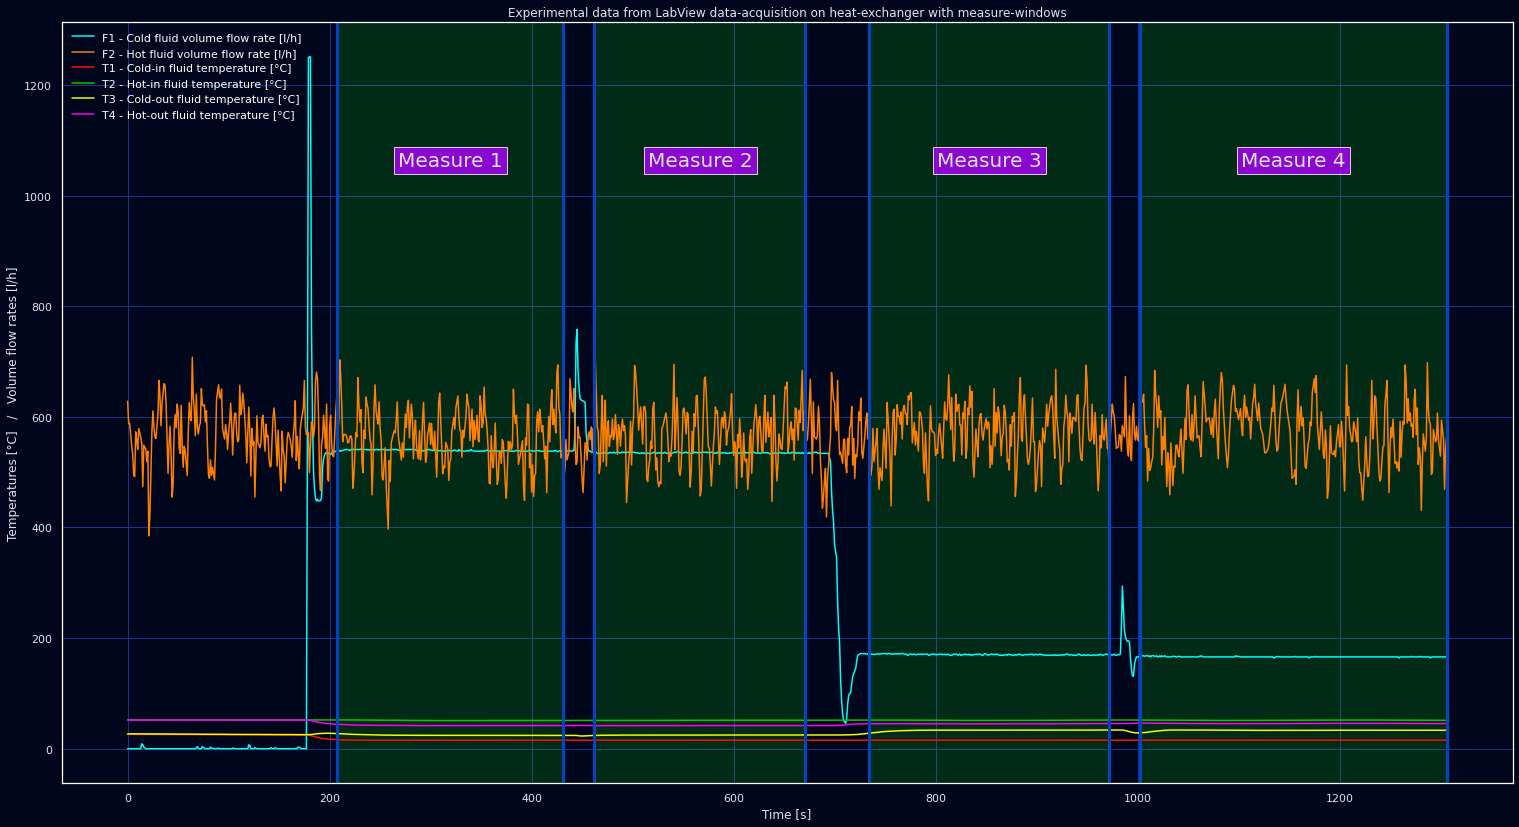
\includegraphics[width=0.9\textwidth]{../final_doc/code_exports/imgs/measures.png}                                        % Size: 100% width of the text
  \caption{\textit{Dati sperimentali analizzati dallo scambiatore di calore e rilevamento delle diverse misure}}            % Image caption
  \label{fig:measures}                                                                                                      % Reference-label to image
\end{figure}                                                                                                                % Figure-end
\begin{figure}[ht!]                                                                                                         % Figure-start
  \centering                                                                                                                % Center image
  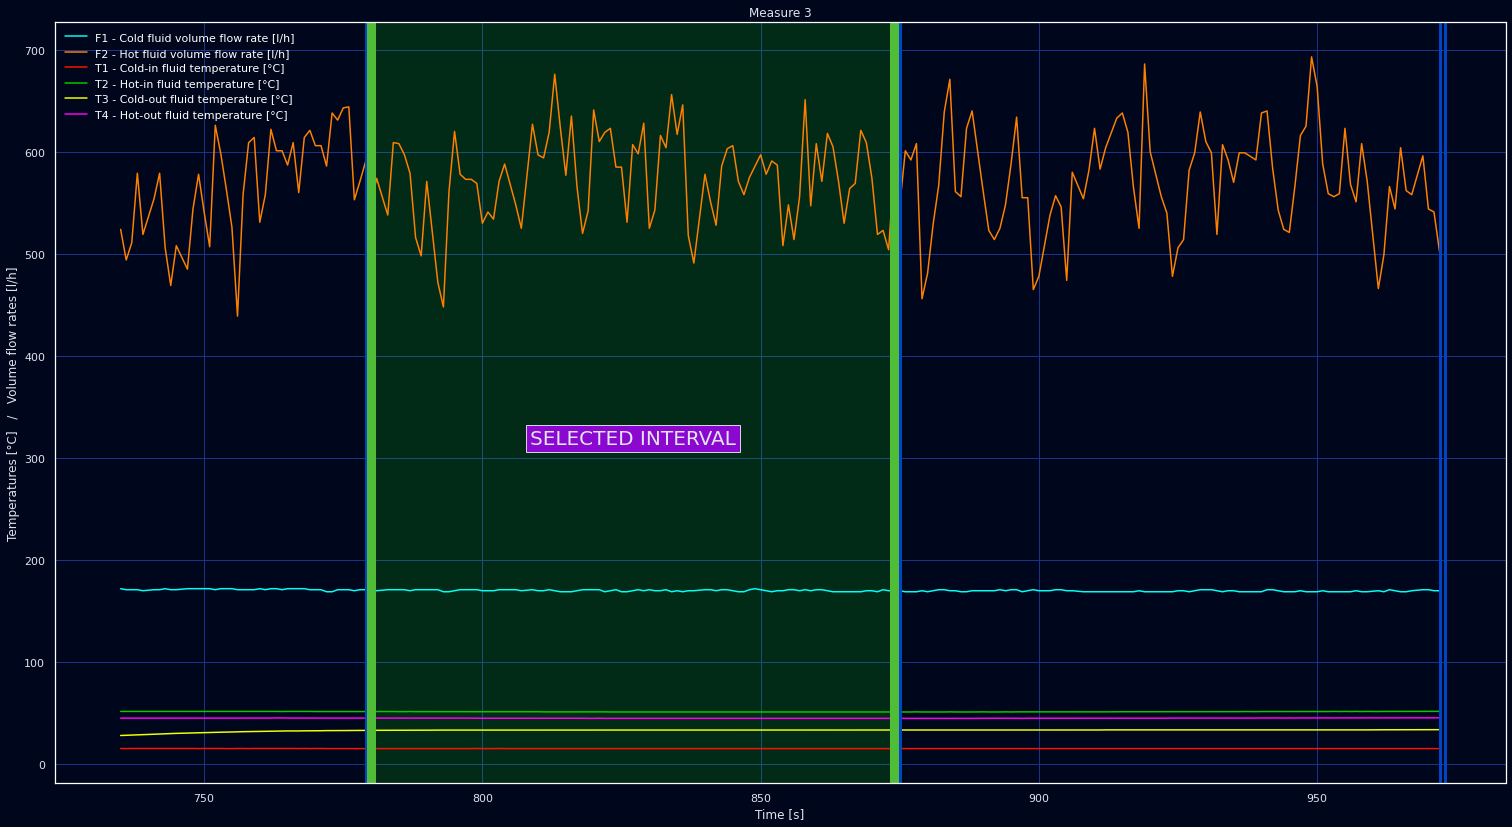
\includegraphics[width=0.9\textwidth]{../final_doc/code_exports/imgs/measure3.png}                                        % Size: 100% width of the text
  \caption{\textit{Scelta del miglior intervallo dati durante la terza misura (ricerca condizioni stazionarie)}}            % Image caption
  \label{fig:measure1}                                                                                                      % Reference-label to image
\end{figure}                                                                                                                % Figure-end
\begin{figure}[ht!]                                                                                                         % Figure-start
  \centering                                                                                                                % Center image
  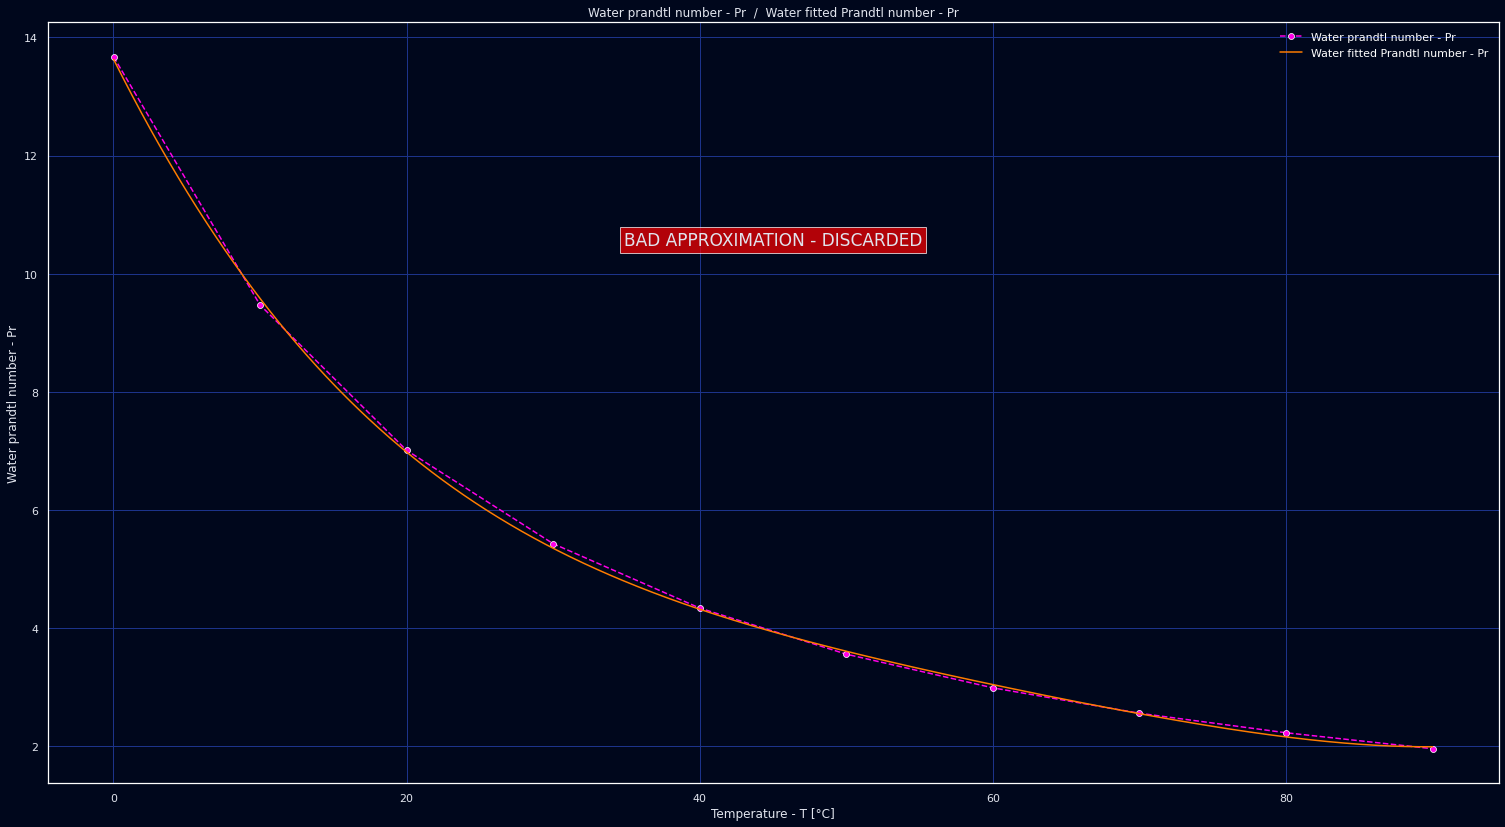
\includegraphics[width=0.9\textwidth]{../final_doc/code_exports/imgs/water_fitted_pr.png}                                 % Size: 100% width of the text
  \caption{\textit{Fitting polinomiale numero di Prandlt acqua (scartato per approssimazione insoddisfacente)}}             % Image caption
  \label{fig:water_fitted_pr}                                                                                               % Reference-label to image
\end{figure}                                                                                                                % Figure-end
\begin{figure}[ht!]                                                                                                         % Figure-start
  \centering                                                                                                                % Center image
  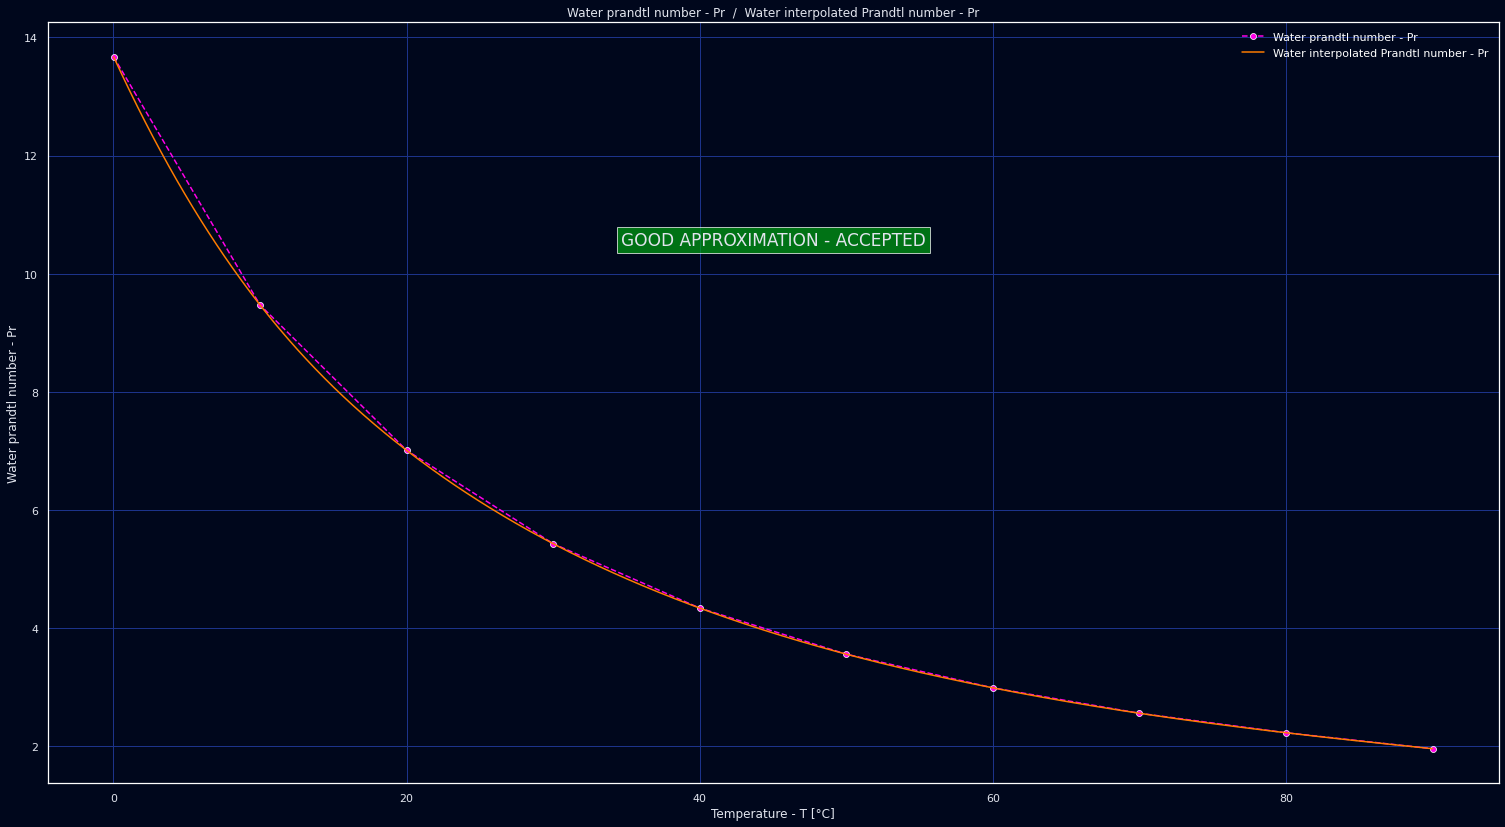
\includegraphics[width=0.9\textwidth]{../final_doc/code_exports/imgs/water_intp_pr.png}                                   % Size: 100% width of the text
  \caption{\textit{Interpolazione polinomiale numero di Prandlt acqua (accettata, buona approssimazione)}}                  % Image caption
  \label{fig:water_intp_pr}                                                                                                 % Reference-label to image
\end{figure}                                                                                                                % Figure-end
\begin{figure}[ht!]                                                                                                         % Figure-start
  \centering                                                                                                                % Center image
  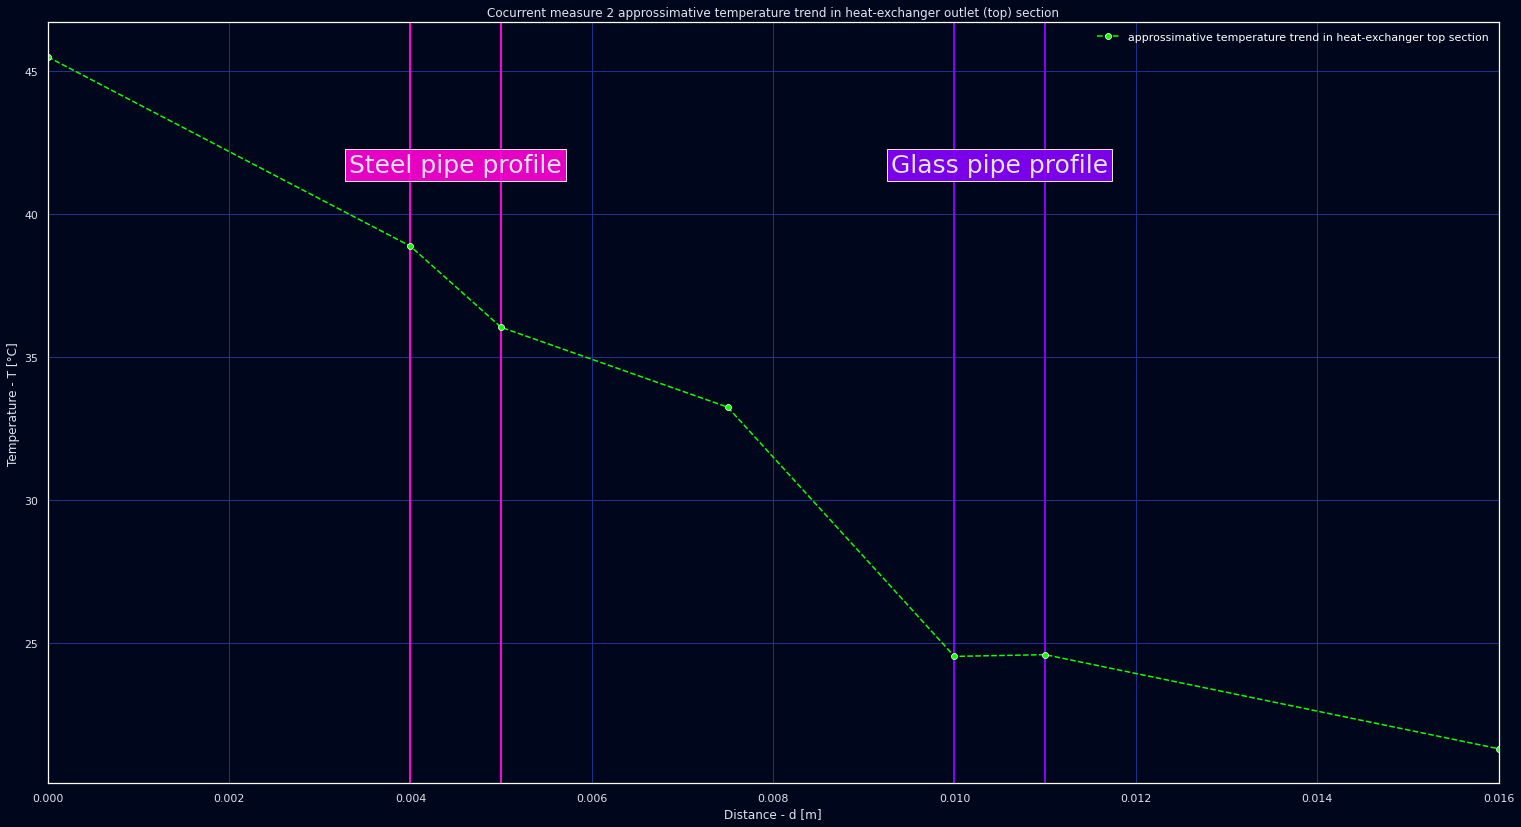
\includegraphics[width=0.9\textwidth]{../final_doc/code_exports/imgs/temp_trend.png}                                      % Size: 100% width of the text
  \caption{\textit{Alcune temperature nella parte superiore dello scambiatore durante la seconda misura in equi-corrente}}  % Image caption
  \label{fig:temp_trend}                                                                                                    % Reference-label to image
\end{figure}                                                                                                                % Figure-end
\begin{figure}[ht!]                                                                                                         % Figure-start
  \centering                                                                                                                % Center image
  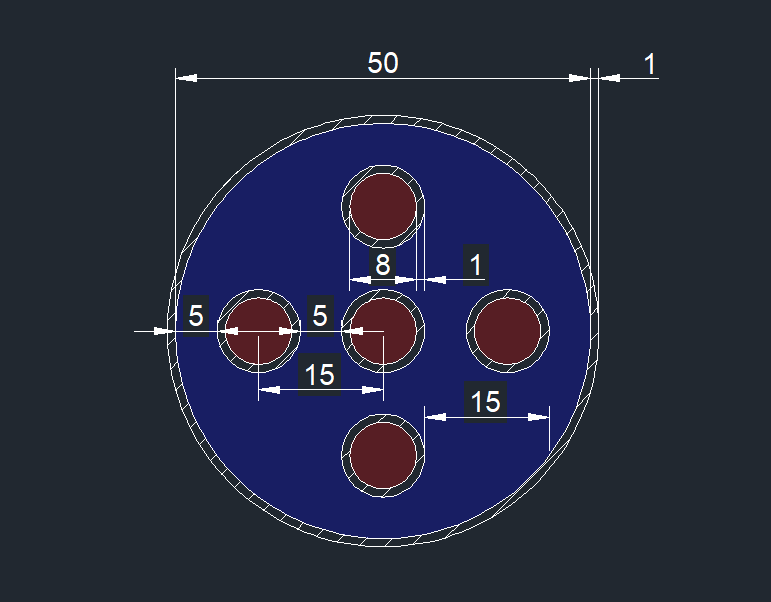
\includegraphics[width=0.75\textwidth]{../final_doc/code_exports/imgs/heat_exchanger.png}                                 % Size: 100% width of the text
  \caption{\textit{Dimensioni scambiatore di calore utilizzate per calcolo dei diametri equivaleti (creata da autocad)}}    % Image caption
  \label{fig:he}                                                                                                            % Reference-label to image
\end{figure}                                                                                                                % Figure-end

\addcontentsline{toc}{section}{Riferimenti bibliografici}                                                                   % Add bibliography inside table of contents
\bibliography{biblio/references}                                                                                            % Bibliography inclusion (biblio/references.bib)

\end{document}                                                                                                              % End document code

%%%%%%%%%%%%%%%%%%%%%%%%%%%%%%%%%%%%%%
%            DOCUMENT END            %                                                                                      % DOC-END
%%%%%%%%%%%%%%%%%%%%%%%%%%%%%%%%%%%%%%
